\documentclass[../main.tex]{subfiles}

\begin{document} %%%%%%%%%%%%%%%%%%%%%%%%%%%%%%%%%%%%%%%%%%%%%%%%%%%%%%%%%%%%
\section{Introducción}

    \begin{definition} \textbf{(Machine Learning)}
        El aprendizaje automático es una parte de la inteligencia artificial y el subcampo de la ciencia de datos. Es una tecnología en crecimiento que permite que las máquinas aprendan de datos anteriores y realicen una tarea determinada automáticamente.
        
        Machine Leaning permite que las computadoras aprendan de las experiencias pasadas por sí mismas, utiliza métodos estadísticos para mejorar el rendimiento y predecir la salida sin ser programado explícitamente. \cite{diferencia_machine_learning_data_science}
    \end{definition}

    \begin{definition} \textbf{(Data Science)}
        Data Science un campo de estudio profundo de los datos que incluye extraer información útil de los datos y procesar esa información utilizando diferentes herramientas, modelos estadísticos y algoritmos de aprendizaje automático

        Es un campo interdisciplinario que utiliza técnicas de análisis de datos, estadística y aprendizaje automático para extraer conocimientos y crear modelos predictivos a partir de grandes conjuntos de datos.
    \end{definition}

    % cargamos imagen
    \begin{figure}[htb]
        \centering
        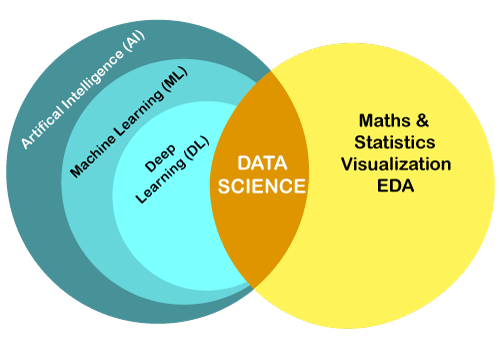
\includegraphics[scale=0.4]{../images/data-science-vs-machine-learning.png}
        \caption{Data Science y Machine Learning}
        \label{fig:data_science_vs_machine_learning}
    \end{figure}

    \subsection{Variables}
        En el contexto del aprendizaje supervisado, se trabaja con \textit{variables independientes} (también conocidas como características, predictores o variables de entrada) y \textit{variables dependientes} (también llamadas variables objetivo o target o variables de salida). Las variables independientes son las que se utilizan para hacer predicciones o estimaciones, mientras que las variables dependientes son los resultados que se intentan predecir o modelar. Por ejemplo, en un problema de predicción de precios de viviendas, las características como el número de habitaciones, la ubicación y el tamaño de la propiedad serían las variables independientes, mientras que el precio de venta sería la variable dependiente.

        \begin{itemize}
            \item Variables Independientes (entradas)
                \begin{itemize}
                    \item Cualitativas
                        \begin{itemize}
                            \item Texto
                                \begin{itemize}
                                    \item Nominales (categorías, Por ejemplo: países, sexo)
                                    \item Ordinales (poco, mucho, muchísimo, Por ejemplo: nivel de tabaquismos)
                                    
                                \end{itemize}
                            \item Númericas
                                \begin{itemize}
                                    \item Nominales
                                    \item Ordinales
                                \end{itemize}
                        \end{itemize}
                    \item Cuantitativas: cuando hablamos de cantidad
                        \begin{itemize}
                            \item Discretas: Por ejemplo año, mes, edad, etc.
                            \item Continuas: Por ejemplo altura, peso, etc.
                        \end{itemize}
                \end{itemize}
            \item Variables Dependientes (salidas, categorías)
        \end{itemize}
        
        \begin{definition}\textbf{(variables cualitativas)} 
            Son aquellas que describen características o cualidades y no pueden ser medidas en términos numéricos. Las variables \textbf{cuantitativas}, por otro lado, son aquellas que pueden ser medidas en términos numéricos y tienen valores numéricos.
        \end{definition}
            
        \begin{definition}\textbf{variables nominales}
            Son aquellas que no tienen un orden natural, como el género o el color de ojos. Las \textbf{variables ordinales} son aquellas que tienen un orden natural, como el nivel de educación (primaria, secundaria, universidad), nivel de tabaquismos: Clasificamos como leve (1), moderado (2), nivel medio (3), importante (4) y muy importante (5).
        \end{definition}
    
        \underline{Variables y tipos de problemas (video 02a min 9:00)}
        \begin{enumerate}
            \item 
                Si la variable dependiente es \textbf{cualitativa}, el tipo de problema es de \textbf{clasificación}. 
            \item 
                Si la variable dependiente es \textbf{cuantitativa}, el problema es de \textbf{regresión}.
                Por ejemplo si quiero predecir el precio de una propiedad.
            \item 
                Si \textbf{NO hay variable} dependientes, el problema es agrupamiento.
        \end{enumerate}
        
        \begin{itemize}
            \item \textbf{Outliers:} Valores atípicos, pueden ser errores o un dato que se sale de la norma.
            \item \textbf{Correlación:} 
                \begin{itemize}
                    \item \textbf{Positiva:} Cuando una variable aumenta la otra también.
                    \item \textbf{Negativa:} Cuando una variable aumenta la otra disminuye.
                    \item \textbf{Sin correlación:} Cuando una variable aumenta la otra no cambia.
                \end{itemize}
            \item \textbf{Varianza:} Es la medida de dispersión de una variable respecto a su media. Si la varianza es alta, los datos están muy dispersos, mientras que si la varianza es baja, los datos están muy agrupados.
            \item \textbf{Covarianza:} Es una medida de la relación lineal entre dos variables aleatorias. Indica cómo varían conjuntamente dos variables aleatorias respecto a sus medias. Si la covarianza es positiva, las variables aumentan o disminuyen conjuntamente, mientras que si la covarianza es negativa, una variable aumenta mientras la otra disminuye.
        \end{itemize}

        % Cargamos una imagen
        \begin{figure}[htb]
            \centering
            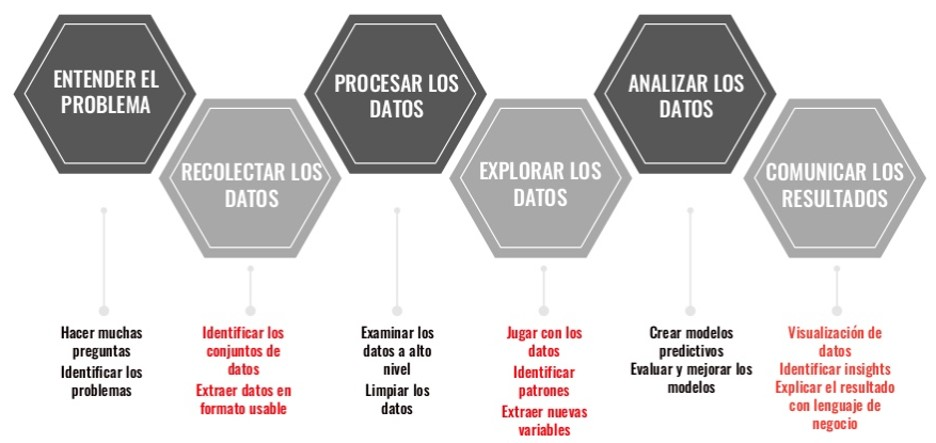
\includegraphics[scale=0.4]{./images/machine.jpg}
            \caption{Metodología de Machine Learning.}
            \label{fig:figura1}
        \end{figure}
    
    \subsection{Formatos de datos y herramientas}
        Ver \href{https://www.youtube.com/watch?v=IIRKrslUO_I&list=PLeo_qKwGPZYevnuxYBfrvQ32zJJE2--Y4&index=6}{Video clase}.
        \begin{enumerate}
            \item \textbf{CSV:} Comma Separated Values. Es un formato de texto plano que se utiliza para almacenar datos tabulares. Cada registro se almacena en una línea y los campos se separan por comas.
            \item \textbf{JSON:} JavaScript Object Notation. Es un formato de texto plano que se utiliza para almacenar datos estructurados. Se utiliza principalmente para transmitir datos entre un servidor y una aplicación web.
            \item \textbf{CSR:} Compressed Sparse Row. Es un formato de matriz dispersa (con gran cantidad de ceros) que se utiliza para almacenar matrices dispersas. Se utiliza principalmente para almacenar matrices dispersas en memoria.
        \end{enumerate}



\end{document}  %%%%%%%%%%%%%%%%%%%%%%%%%%%%%%%%%%%%%%%%%%%%%%%%%%%%%%%%%%%%%